\documentclass[hyperref=colorlinks]{beamer}
\mode<presentation>
\usetheme{iclpt}
\setbeamertemplate{navigation symbols}{}
\setbeamertemplate{headline}{
\begin{beamercolorbox}[leftskip=.2cm,rightskip=.2cm,topskip=.2cm,ht=1.1cm,dp=0.1cm,wd=\textwidth]{institute in head/foot}
  
\includegraphics[height=1cm]{icl.pdf}
  \hfill
  
\includegraphics[height=1cm]{../Pics/CMS-Color.pdf}
\end{beamercolorbox}
}
\setbeamertemplate{footline}{
\begin{beamercolorbox}[ht=.55cm,dp=0.4cm,wd=\textwidth,leftskip=.3cm]{author in head/foot}%
  \begin{minipage}[c]{5cm}%
    \usebeamerfont{author in head/foot}
    \insertshortauthor 
    \insertshorttitle
    \end{minipage}\hfill%
  \insertframenumber{} / \pageref{lastframe}
  \hfill
  \begin{minipage}{6cm}
    \hfill
  \end{minipage}
\end{beamercolorbox}%
}

\usepackage{color}
\usepackage{tabularx,colortbl}
\usepackage{graphicx}
\usepackage{pdfpages}
\usepackage{feynmp}
\usepackage{multirow}
\DeclareGraphicsRule{*}{mps}{*}{}

\title{\vspace{-0.2cm} Higgs to Invisible Combinations}
\subtitle{Run I legacy result: HIG-15-012 \\ Contributing analyses: HIG-13-030, HIG-14-038, EXO-12-055}
\author[P. Dunne]{\underline{P. Dunne} on behalf of the H$\rightarrow$invisible analysis groups}
\titlegraphic{
  \vspace{-0.7cm}
  %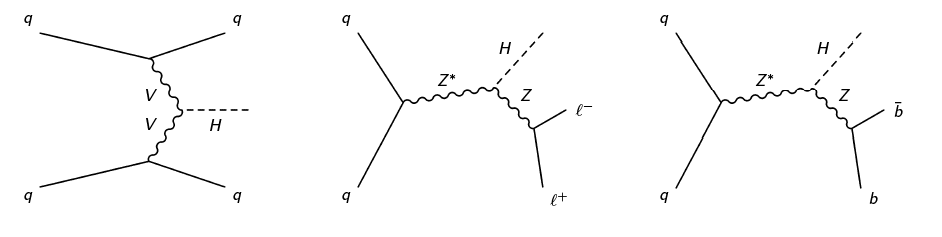
\includegraphics[width=\textwidth]{TalkPics/invcomb021213/feyndiags}
%% \begin{fmfgraph*}(100,70)
%%         \fmfleft{i1,i2}
%%         \fmfright{o1,o2,o3}
%%         \fmf{fermion}{i1,v1,o1}
%%         \fmf{fermion}{i2,v2,o3}
%%         \fmf{phantom,tension=4/5}{v1,v2}
%%         \fmffreeze
%%         \fmf{photon,label=$W,,Z$}{v1,v3}
%%         \fmf{photon,label=$W,,Z$}{v2,v3}
%%         \fmf{dashes}{v3,o2}
%%         \fmflabel{$q$}{i1}
%%         \fmflabel{$q$}{i2}
%%         \fmflabel{$q$}{o1}
%%         \fmflabel{$q$}{o3}
%%         \fmflabel{$H$}{o2}
%%       \end{fmfgraph*}
}
\date{}
\begin{document}
\begin{fmffile}{hig15012preapprovalfeyndiags}

%TITLE PAGE
\section{Title}
\begin{frame}
  \titlepage
  
\end{frame}

%!!CLOSURE TEST STATEMENT PU jet ID
%OUTLINE
\begin{frame}
      \scriptsize
  \begin{columns}
    \column{.65\textwidth}
    \vspace{-.2cm}
    \begin{block}{\footnotesize Run I Reminder}
      \begin{itemize}
      \item Run 1 Prompt data searches in  Z($\ell\ell$)H, Z(bb)H and VBF channels published in HIG-13-030
      \item VBF parked update and EXO-12-055 added for HIG-15-012
      \item 95\% C.L. observed (expected) limit 36 (30) \%
      \end{itemize}
      \end{block}
    \begin{block}{\footnotesize Run II}
      \begin{itemize}
      \item Run I legacy Higgs uncertainties can still accommodate significant BSM properties
      \item Invisible group has good integration with combination group
      \item We must make sure we retain the orthogonality of the channels we achieved in run I
      \end{itemize}
    \end{block}
    \vspace{-.2cm}
    \column{.45\textwidth}
    \centering
    \begin{fmfgraph*}(80,50)
      \fmfleft{i1,i2}
      \fmfright{o1,o2,o3}
      \fmf{fermion}{i1,v1,o1}
      \fmf{fermion}{i2,v2,o3}
      \fmf{phantom,tension=4/5}{v1,v2}
      \fmffreeze
      \fmf{photon}{v1,v3}
      \fmf{photon}{v2,v3}
      \fmf{dashes}{v3,o2}
      \fmflabel{$q$}{i1}
      \fmflabel{$q$}{i2}
      \fmflabel{$q$}{o1}
      \fmflabel{$q$}{o3}
      \fmflabel{$H$}{o2}
    \end{fmfgraph*}

    \vspace{.6cm}

    \begin{fmfgraph*}(80,50)
      \fmfleft{i1,i2,ix,i3,iy,i4,i5}
      \fmfright{o1,o2,ox,o3,oy,o4,o5}
      \fmf{phantom}{i2,v1,o2}
      \fmf{phantom}{i4,v2,o4}
      \fmffreeze
      \fmf{gluon}{i2,v1}
      \fmf{gluon}{i4,v2}
      \fmf{phantom}{v1,v4,v3,v5,v2,v1}
      \fmf{fermion}{v1,v3,v2,v1}
      \fmf{dashes,tension=8/5}{v3,o3}
      \fmffreeze
      \fmf{gluon}{v4,o2}
      \fmflabel{$g$}{i2}
      \fmflabel{$g$}{i4}
      \fmflabel{$H$}{o3}
      \fmflabel{$jet$}{o2}
    \end{fmfgraph*}

    \vspace{.6cm}

    \begin{fmfgraph*}(80,50)
      \fmfleft{i1,i2}
      \fmfright{o1,o2,o3}
      \fmf{fermion}{i1,v1,i2}
      \fmf{photon}{v1,v2,o1}
      \fmf{dashes}{v2,o3}
      \fmflabel{$q$}{i1}
      \fmflabel{$q$}{i2}
      \fmflabel{$Z$}{o1}
      \fmflabel{$H$}{o3}
    \end{fmfgraph*}

    
    \end{columns}
\end{frame}

\begin{frame}
  \label{lastframe}
  \frametitle{Results - by production mode tag}
  \centering
  \scriptsize
  \vspace{-.3cm}
  \begin{block}{}
    \begin{itemize}
    \item We gain significantly from combination of all analyses
    \item VBF tagged is VBF analysis
    \item VH-tagged is Z(ll)H + Z(bb)H + boosted and resolved from monojet+V(had)H
    \item ggH-tagged is monojet from monojet+V(had)H
    \end{itemize}
  \end{block}
  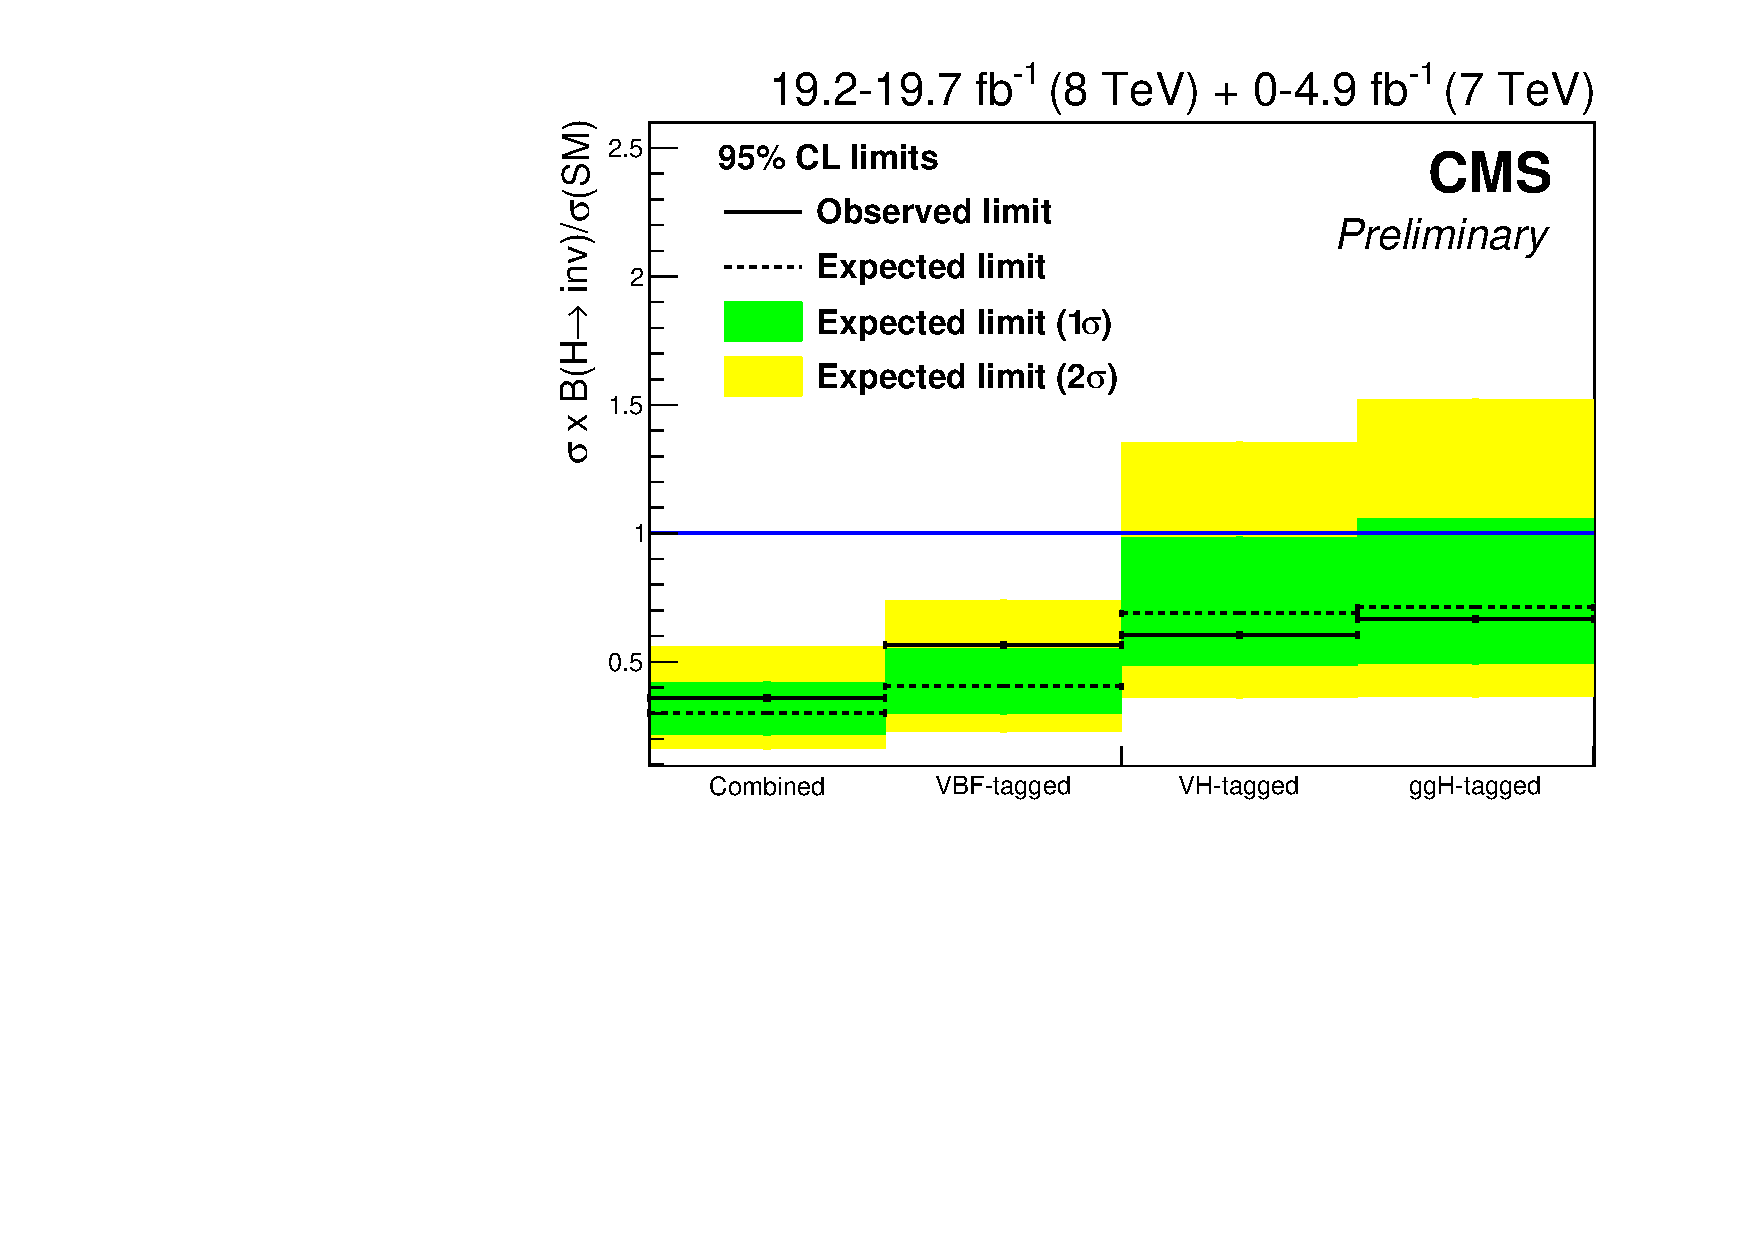
\includegraphics[width=.64\textwidth]{TalkPics/hig15012approval/channellimit.pdf}

\end{frame}

%UPDATED BACKUP
\begin{frame}
  \frametitle{Backup}
\end{frame}

\begin{frame}
  \frametitle{Limits}
  \scriptsize
  \begin{block}{}
    \begin{itemize}
    \item 95\% CL upper limits set using asymptotic method in combine assuming SM Higgs boson production and acceptance
    \end{itemize}

    \centering
    \begin{tabular}{lc}
       \hline
       \hline
       \multirow{2}{*}{Channel}        & Observed (expected) upper \\
       & limits on $\frac{\sigma}{\sigma_{SM}}\cdot$B(H$\rightarrow$inv) (\%) \\
       \hline
       \hline
       VBF & 57 (40) \\
       Monojet+V(had)H & 54 (62) \\
       Z(ll)H                & 83 (86)       \\
       Z(bb)H                & 182 (199)     \\
        \hline
       Combined                & \textcolor{red}{36} (30)       \\
       \hline
       \hline
  \end{tabular}

  \end{block}

\end{frame}



%THEORY MOTIVATION
\begin{frame}
    \frametitle{Why Higgs to Invisible?}
    \vspace{-.2cm}
    \begin{columns}
      \column{.5\textwidth}
      \begin{block}{\scriptsize Experimental motivation}
        \scriptsize
        \begin{itemize}
        \item Current measurements of the 125 GeV Higgs boson are compatible with Standard Model (SM) expectations
        \item[-] large uncertainties can still accommodate significant beyond the SM (BSM) properties
        \item Additional Higgs bosons with exotic decays are not excluded
        \end{itemize}
      \end{block}
      \column{.45\textwidth}
      \hfill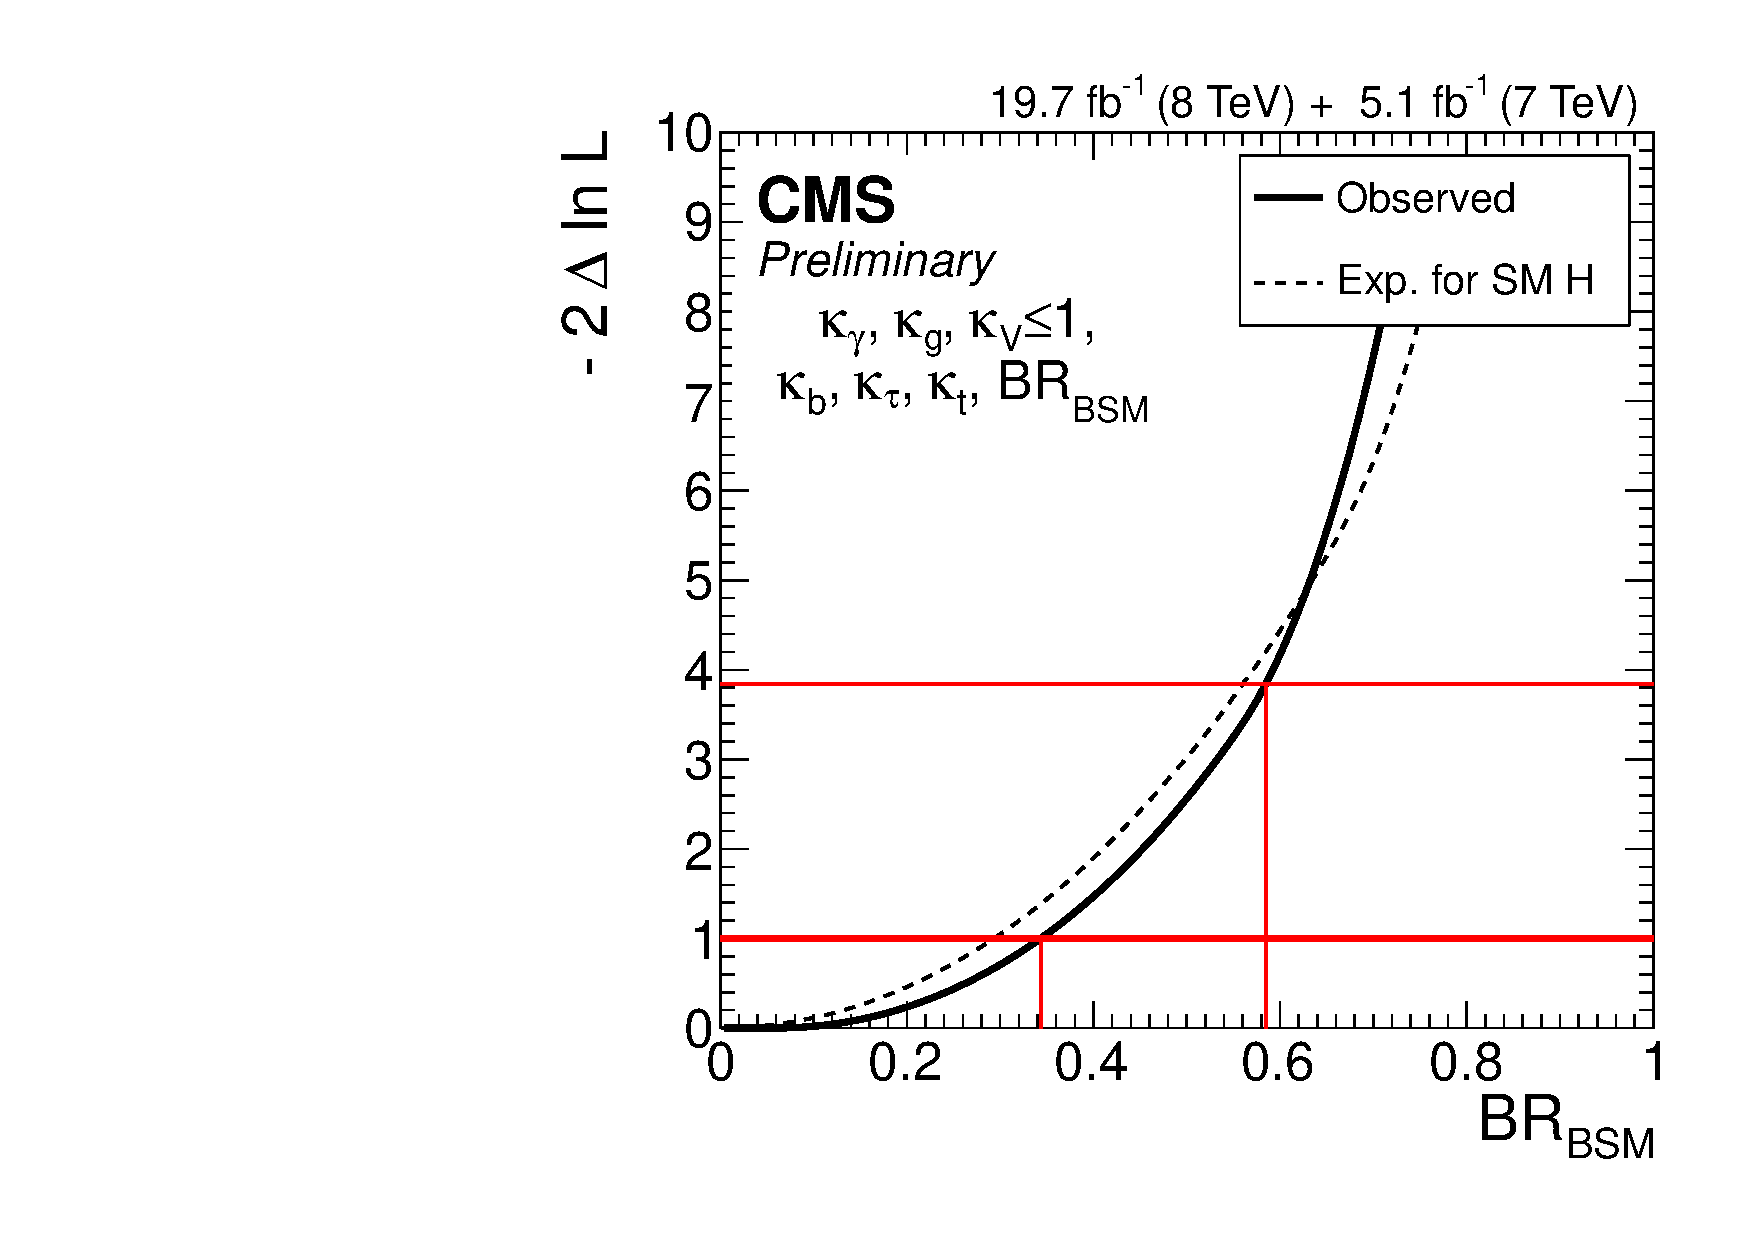
\includegraphics[height=.55\textheight]{TalkPics/panicpics/indirectbrbsm.pdf}
      \column{.05\textwidth}
    \end{columns}
    \begin{columns}
      \column{1.095\textwidth}
      \begin{block}{\scriptsize Theoretical motivation}
        \scriptsize
        \begin{itemize}
        \item Many BSM theories predict Higgs boson decays to invisible final states:
        \item[-] e.g. SUSY, extra dimensions, fourth-generation neutrinos
        \item These final state particles are often dark matter candidates
        \end{itemize}
      \end{block}
    \end{columns}

  \end{frame}

\end{fmffile}
\end{document}
